

\chapter{The Net Carbon Impact of this PhD}\label{ch:impact}

In this short concluding Chapter, I will estimate the \ch{CO2} emitted (Section \ref{sec:burning}) and, with much more uncertainty, the expectation value of the \ch{CO2} saved during my PhD project (Section \ref{sec:millivolt}). The idea is to determine whether I have done any net good during the past three years with respect to the climate crisis described in Chapter 1.

A version of this question, rearranged to be a bit more rigorous, is:
\begin{question}
	What portion of a millivolt's improvement in efficiency of PEM electrolyzers worldwide in the year 2030 would have to be attributable to my research in order to offset the \ch{CO2} footprint of my PhD project? \label{q:impact}
\end{question}

Finally, the last Section will serve as a conclusion and outlook for this Thesis.


\section{Burning}\label{sec:burning}

I have had the fantastic opportunity of working with scientists all over the world during this PhD project. I owe thanks for these opportunities to our wide network of collaborators as well as the EtiteForsk Travel Grant that I was awarded by the Danish Ministry for Higher Education and Science in 2018. (I have been especially quick to take opportunities to travel to the United States, since I also visited friends and family on those trips.)

Figure \ref{fig:flying} shows the institutes that I have visited and conferences that I have attended during the three years of my PhD on a map of the world. The routes that I have flown are shown together with their distance and the number of times that I flew that route.

While grateful for all of these opportunites, I am not proud of how much I have been traveling, and plan on much less air travel in the future. Each trip has come with an environmental cost, since air travel is the most \ch{CO2}-intensive activity an individual can choose to do.

\begin{figure}[h!]
	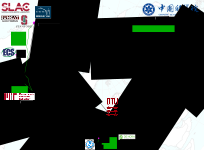
\includegraphics[width=\textwidth]{05_Impact/fig/flying.png}
	\caption{Map of research collaborations, conferences, and flights during this PhD project, superimposed on a map of the northern hemisphere. Flights are indicated as black lines, and the distance and total number of one-way flights I took over the three-year period September 2016-August 2019 are indicated. The projects requiring the most traveling have been beamline experiments at SLAC in California (Paper \ref{Scott2019_GIXRD}) and the collaboration with the Chinese Academy of Sciences (CAS) in Fuzhou, Fujian, China.}
	\label{fig:flying}
\end{figure}

Adding up all of the trips in Figure \ref{fig:flying}, I have flown 187600 km during this PhD project, equivalent to circling the earth 4.7 times at the equator. Using an average greenhouse gas emissions of 0.19 kg \ch{CO2} equivalents per passenger per kilometer\cite{Larsson2018}, this is 36 tons of \ch{CO2}, or 12 tons of \ch{CO2} per year (3.2 tC/yr). This is actually a slight underestimation, since it uses the direct-flight distances, whereas most of the trips indicated involved at least one transfer.

Domestic \ch{CO2} emissions per capita in Denmark in 2017 were 6.1 tons of \ch{CO2} per year\cite{Ritchie2019a} (1.7 tC/yr), so the flying alone during my PhD project represents approximately twice the average person's \ch{CO2} emissions in Denmark during the same period. 

There are numerous sources of \ch{CO2} emissions associated with the lab work of my PhD project. The only one considered here, which I believe to be the most significant, is that associated with electricity usage. The carbon footprint of equipment, chemicals, water, and consumables, for example, is not considered. Building 312 at DTU houses approximately 12 vacuum setups in active use including the EC-MS setup, which was the primary tool of my PhD project. The setup includes two roughing pumps, two turbo pumps, a large electronics rack, three computers and a number of control elements, and is left on 24 hours a day, 7 days a week. Others have used the EC-MS setup, and I have also used other setups, so taking responsibility for 1/12 of the hall's \ch{CO2} emissions seems a fair average. The heating (771 MWh) + electricity (162 MWh) used by building 312 in 2017 was 933 MWh. The carbon intensity of electricity generation in Denmark in 2017 was 291 kg \ch{CO2} per MWh of electricity\cite{DanishEnergyAgency}. Extrapolating to the 3-year PhD project, the \ch{CO2} cost of my lab work has been:
\begin{equation}
3 \text{[yr]} \cdot \frac{1}{12} \cdot 291 \left[\frac{\text{kg}_{\ch{CO2}}}{\text{MWh}}\right] \cdot 933\text{[MWh]} = 68 [\text{t}_{\ch{CO2}}]\,,
\end{equation}
which is 22.6 tons of \ch{CO2} per year (6.2tC/yr). This is a slight overestimation as I have assumed that the carbon intensity of heat is equal to that of electricity, when actually it is lower \cite{EnergiNet}. 

The \ch{CO2} cost of running the EC-MS setup is thus, surprisingly, even higher than the \ch{CO2} cost of the flying I have done during my PhD project. This would likely not be the case in the future, as progress in decarbonizing electricity is much faster than progress in decarbonizing aviation (see Chapter \ref{ch:Intro}). 

Adding the costs up my setup, travel, and living as an average Dane (probably an overestimation, as I have a vegetarian cyclist lifestyle when not traveling), the \ch{CO2} cost of my 3-year PhD project is approximately:
\begin{equation}
c = c_\text{el} + c_\text{travel} + c_\text{live} = 68 [\text{t}_{\ch{CO2}}] + 36 [\text{t}_{\ch{CO2}}] + 3 \text{[yr]} \cdot 6.1  [\text{t}_{\ch{CO2}}/\text{yr}] = 122 [\text{t}_{\ch{CO2}}]\label{eq:costs}
\end{equation}
That is the debt I have to pay, before I can even begin to claim that I'm helping to solve the climate crisis.






\section{How much difference a millivolt makes}\label{sec:millivolt}



\section{Conclusion}\label{sec:conclusion}


\subsection*{The Project}

Chapter \ref{ch:Intro} described how greenhouse gas emissions need to be cut fast to avoid disasterous and worsening effects of climate change. To be in line with the ambitions of the Paris agreement, societies should cut emissions to half or less by 2030. In order for progress being made in wind and solar energy to drive sufficient overall emissions reductions, technological solutions are needed to keep the lights on when the wind isn't blowing and the sun isn't shining, and to spread the decarbonization to other sectors including transport and industry. Water electrolysis to make hydrogen for energy storage, fuel, and industrial reactant has the potential to help with all of these needs.

The goal of this PhD project has been to use in-situ techniques to better understand the fundamentals of a number electrocatalytic reactions. I've had the chance to work on the propene oxidation reaction (Paper \ref{Winiwarter2019}), the \ch{CO2} and \ch{CO} reduction reactions (Papers \ref{Scott2019_GIXRD}, \ref{Nitopi2019}), and the hydrogen evolution reaction (Paper \ref{Scott_Engstfeld2019}). However, this Thesis has focused on the oxygen evolution reaction (OER, Papers \ref{Roy2018} and \ref{Scott_Rao2019}). The OER, as the main source of efficiency loss in water electrolysis cells, and as a required counter-reaction for any other fuel-producing electrochemical process, is arguably the most important electrochemical reaction to understand and improve.

\subsection*{EC-MS and isotopes}

The tool I've used for most of the work in this PhD project is chip electrochemistry - mass spectrometry, described in Paper \ref{Trimarco2018}. This technique uses a microscopic sampling volume in a silicon microchip to saturate the electrolyte with inert or reactant gas, and to deliver any evolved gases to the vacuum chamber containing the mass spectrometer. This setup is highly sensitive and features well-controlled mass transport, making it ideal for fundamental studies. (Section \ref{sec:ECMS})

%Two model experiments - RHE potential measurement by saturating the electrolyte at a platinum electrode with \ch{H2}, and CO stripping - were shown first in isotopically natural electrolyte and then in isotope-labeled electrolyte. When a platinum electrode is simultaneously in contact with \ch{D2O}-labeled electrolyte and \ch{H2} and open-circuit potential, the evolved \ch{D2} gives a measure of the rate at which the forward and backwards reactions are happening at equilibrium. This experiment will, however, have to be repeated under conditions which are not dominated by mass transport. When \ch{C^{16}O} is oxidized in \ch{H2^{18}O}-containing electrolyte, it forms \ch{C^{16}O^{18}O}, as expected when one oxygen comes from \ch{CO} and one from \ch{H2O}. However, a \ch{C^{18}O2} signal follows, caused by oxygen switching between \ch{CO2} and \ch{H2O} via carbonic acid. The rate of change of the \ch{C^{18}O^{16}O} to \ch{C^{18}O2} ratio can be used to calculate the forward rate constant of the aqueous \ch{CO2} - carbonic acid equilibrium. 

Isotope-labeling, which enables the tracking of atoms, is a powerful strategy in catalysis, including electro-catalysis. An experiment that illustrates the possibilities of using chip EC-MS together with isotope labeling is one which confirms the Langmuir-Hinshelwood mechanism for CO electro-oxidation. If a sample with an \ch{^{18}O}-labeled surface oxide layer is reduced in \ch{C^{16}O}-saturated \ch{H2^{16}O} electrolyte, there is a transient of \ch{C^{16}O^{18}O} which is formed. This is when \ch{$*$ ^{18}O} on the surface of the oxide is reduced to \ch{$*$ ^{18}OH} which reacts with adsorbed \ch{$*$ ^{16}O}. This experiment can also confirm that a labeled oxide layer is still present in a sample if it is not evolved as \ch{^{16}O^{18}O} during OER.  (Section \ref{subsec:extraction})

\subsection*{Oxygen evolution experiments}

Checking for incorporation of lattice oxygen in evolved \ch{O2} by isotope-labeling is an experiment often used to gain insight into the OER mechanism on electrocatalyst materials (Section \ref{sec:lattice_O}). Such experiments, with a lot of trial and error, have also been an important part of my PhD project. From the literature and from the experience of my own studies, I conclude that the best way to do these experiments is to prepare the OER catalyst with full \ch{^{18}O} labeling and test in un-labeled electrolyte using a constant-current period of oxygen generation. A control sample which has the natural ratio should be tested first, to ensure that the m/z=32, m/z=34, and m/z=36 signals are as expected by the natural \ch{O2} isotopic distribution. Any excess m/z=34 or m/z=36 signal in the lattice oxygen evolution experiment should be quantified to get the absolute number of lattice oxygen atoms evolved. The electrolyte used for the isotope exchange experiment should be collected and analyzed by ICP-MS, so that the number of metal atoms dissolved can be compared quantitatively to the number of lattice oxygen atoms evolved. Only if lattice oxygen evolution exceeds metal dissolution can it be concluded that lattice oxygen exchange is part of the catalytic OER mechanism and not a degradation side-process. Finally, the isotopic composition of the electrocatalyst surface after oxygen evolution should be checked - in a truly catalytic process, \ch{^{16}O} should be incorporated into the catalyst. (Section \ref{sec:dissolving})

Along the way to this procedure, we concluded in Paper \ref{Roy2018} that nickel-iron based electrocatalysts in alkaline electrolyte do not evolve lattice oxygen. Using the recommended procedure, we showed that labeled ruthenium dioxide (\ch{Ru^{18}O2}) evolves some lattice oxygen but that it is most likely due to a degradation, and not a catalytic, mechanism. Labeled iridium dioxide (\ch{Ir^{18}O2}), on the other hand, does show a minor catalytic OER mechanism involving lattice oxygen exchange, but it amounts to only one ten-thousandth of the total evolved oxygen. This can only be detected because of the control and sensitivity enabled by the chip EC-MS method.

This sensitivity also allows us to observe oxygen evolution at low overpotential, where other process may mask it in the electrode current. On a high-surface-area ruthenium foam, we observe catalytic \ch{O2} evolution down to 1.29 V vs RHE, a record to the best of our knowledge, though the rates are tiny, i.e., a TOF of 10$^{-7}$ s$^{-1}$. The TOF of ruthenium foam together with a series of sputtered \ch{RuO2} films tested the same way fall on a shared TOF-vs-potential curve which we measured over seven orders of magnitude. This curve has a high and increasing potential dependence at very low overpotentials, which we hope will be useful input for rational OER catalyst design. (Section \ref{sec:low_O2})

\subsection*{Net \ch{CO2} impact}

But does all this work do any good? This is the question that the previous two Sections of this final Chapter have sought to answer. The question was simplified to consider only one metric: net \ch{CO2}; and to only consider one effect: an improvement in water oxidation efficiency. This PhD project has been a \ch{CO2}-intensive one due to a lot of traveling and high electricity consumption of the chip EC-MS setup. However, using results from an energy systems model of Europe for the year 2030, I found that the approximately 122 tons of \ch{CO2} emitted during this PhD are avoided in one year (the year 2030) if they can be attributed just an 0.03 mV improvement in the OER overpotential of electrolysis cells.

Since the results presented here have a non-zero chance of contributing to a breakthrough worth much more than that, I think this is not too optimistic an expectation value. Furthermore, this is without taking into account the value of the other projects and of the education, both my own education and the teaching and supervising I have done as part of this PhD program. I think it is therefore highly likely that this PhD project has done net good. There are, of course, lots of uncertainties involved - even in the aspect of my research that I chose for this calculation because I thought it the least uncertain. However, I think it could be good practice to consider, informally, how to maximize the net \ch{CO2} benefit of research projects.


\label{sec:conclusion}